%25/02/2026
\section{Approssimazione di funzioni}
\subsection{Interpolazione polinomiale}

Dal punto di vista geometrico, abbiamo la seguente situazione:

\begin{center}
\begin{tikzpicture}[scale=1.2]
    % Assi
    \draw[->, thick] (0,0) -- (10,0) node[right] {$x$};
    \draw[->, thick] (0,0) -- (0,5);
    
    % Punti sull'asse x
    \draw (1,0) node[below] {$x_0$} -- (1,0.1);
    \draw (3,0) node[below] {$x_1$} -- (3,0.1);
    \draw (5,0) node[below] {$x_2$} -- (5,0.1);
    \node at (6.5, -0.3) {$\dots$};
    \draw (8.5,0) node[below] {$x_n$} -- (8.5,0.1);
    
    % Funzione f(x)
    \draw[blue, thick] (1,1.5) to[out=45, in=190] (3,2.5) to[out=10, in=180] (5,2.8) to[out=0, in=200] (8.5, 4.5) node[below right] {$f(x)$};
    
    % Polinomio interpolante
    \draw[orange, thick] (1,1.5) to[out=10, in=200] (3,2.5) to[out=45, in=170] (5,2.8) to[out=-10, in=220] (8.5, 4.5);
    
    % Linee tratteggiate e punti rossi
    \draw[dashed, red] (1,0) -- (1,1.5);
    \fill[red] (1,1.5) circle (1.5pt);
    
    \draw[dashed, red] (3,0) -- (3,2.5);
    \fill[red] (3,2.5) circle (1.5pt);
    
    \draw[dashed, red] (5,0) -- (5,2.8);
    \fill[red] (5,2.8) circle (1.5pt);
    
    \draw[dashed, red] (8.5,0) -- (8.5,4.5);
    \fill[red] (8.5,4.5) circle (1.5pt);
\end{tikzpicture}
\end{center}

Data una funzione $f:[a,b]\rightarrow \mathbb{R}$, e $n+1$ ascisse distinte nell'intervallo $[a,b]$, $a \le x_0 < x_1 < \dots < x_n \le b$,  in cui è noto il valore della funzione $f(x)$. Ovvero sono assegnate $n+1$ coppie di dati $(x_i, f_i)$, dove $f_i \equiv f(x_i)$, per $i=0,\dots,n$.

\textbf{Obiettivo}: costruire una funzione ``semplice'' che interpola i dati $(x_i, f_i)$. A riguardo, considereremo tra le varie possibilità, funzioni interpolanti che sono polinomi.

\begin{definition}
Diremo che $p(x) \in \Pi_n$ è il polinomio interpolante le coppie di dati $(x_i, f_i)$ per $i=0,\dots,n$ se $p(x_i) = f_i$ per $i=0,\dots,n$.
\end{definition}

Vale a riguardo il seguente risultato.

\begin{teorema}
Date le $n+1$ coppie di dati $(x_i, f_i)$ per $i=0,\dots,n$ con $x_i \neq x_j$ se $i \neq j$ (ascisse distinte), allora esiste ed è unico $p(x) \in \Pi_n$ tale che $p(x_i) = f_i$ per $i=0,\dots,n$.
\end{teorema}

\begin{proof}
Se $p(x) \in \Pi_n$, allora sarà della forma:
$$p(x) = \sum_{k=0}^{n} a_k x^k \quad (1)$$
dove $a_0, \dots, a_n$ sono i coefficienti (per il momento incogniti) della rappresentazione di $p(x)$ rispetto alla base delle potenze $(x^0, x^1, \dots, x^n)$. 

I coefficienti si otterranno imponendo le condizioni di interpolazione:
$$p(x_i) = \sum_{k=0}^{n} a_k x_i^k = f_i, \quad i=0,\dots,n$$
ovvero:
\begin{align*}
x_0^0 a_0 + x_0^1 a_1 + \dots + x_0^n a_n &= f_0 \\
x_1^0 a_0 + x_1^1 a_1 + \dots + x_1^n a_n &= f_1 \\
&\dots \\
x_n^0 a_0 + x_n^1 a_1 + \dots + x_n^n a_n &= f_n
\end{align*}
che è un sistema di $n+1$ equazioni lineari nelle $n+1$ incognite $a_0, \dots, a_n$. Pertanto la sua soluzione esisterà ed è unica se e solo se la matrice dei coefficienti è non singolare.

Se definiamo il vettore delle incognite $\underline{a} = [a_0, a_1, \dots, a_n]^T \in \mathbb{R}^{n+1}$ e quello dei termini noti $\underline{b} = [f_0, f_1, \dots, f_n]^T \in \mathbb{R}^{n+1}$, allora il sistema lineare (1) si può scrivere in forma vettoriale come:
$$V \underline{a} = \underline{b} \quad (2)$$
con:
$$V = \begin{bmatrix}
1 & x_0 & \dots & x_0^n \\
1 & x_1 & \dots & x_1^n \\
\vdots & \vdots & \ddots & \vdots \\
1 & x_n & \dots & x_n^n
\end{bmatrix} \in \mathbb{R}^{(n+1) \times (n+1)}$$

$V$ è la matrice di Vandermonde, molto nota in Analisi Numerica. In particolare, si capisce che:
$$\det(V) = \prod_{i>j} (x_i - x_j) \neq 0$$
poiché le ascisse sono, per ipotesi, tutte tra loro distinte. Pertanto, la soluzione di (2) esiste ed è unica, ovvero esiste ed è unico il polinomio $p(x) \in \Pi_n$ interpolante le coppie di dati.
\end{proof}

\textbf{Osservazione}: Osserviamo che, tuttavia, il calcolo del polinomio interpolante mediante la risoluzione del sistema lineare (2) non è una buona prassi computazionale. Questo è dovuto al fatto che il numero di condizionamento della matrice $V$ cresce rapidamente al crescere di $n$. 

Ad esempio, se prendiamo $x_i = i/n$ ascisse equidistanti, otteniamo dei numeri di questo tipo:

\begin{center}
\begin{tabular}{|c|c|c|c|c|}
\hline
$n$ & 2 & 3 & 5 & 10 \\
\hline
$K(V)$ & $\sim 15$ & $\sim 100$ & $\sim 5 \cdot 10^3$ & $\sim 10^{17}$ \\
\hline
\end{tabular}
\end{center}

\textit{Esercizio}: calcolare la precedente tabella (\texttt{help vander}).

\vspace{0.5cm}
\textbf{Svolgimento dell'esercizio (GEMINI):}

Per verificare la rapida crescita del numero di condizionamento $K(V)$ della matrice di Vandermonde al variare di $n$, possiamo scrivere un semplice script in MATLAB o GNU Octave. 

Il comando \texttt{vander(x)} genera la matrice associata al vettore delle ascisse \texttt{x}, mentre \texttt{cond(V)} ne calcola il numero di condizionamento in norma 2. Ricordiamo che per un polinomio di grado $n$, abbiamo bisogno di $n+1$ punti (ascisse).

\begin{verbatim}
% Vettori dei gradi n richiesti
n_val = [2, 3, 5, 10];

fprintf(' n | Condizionamento K(V)\n');
fprintf('-------------------------\n');

for i = 1:length(n_val)
    n = n_val(i);
    
    % Creazione di n+1 ascisse equidistanti nell'intervallo [0, 1]
    x = (0:n)/n; 
    
    % Creazione della matrice di Vandermonde
    V = vander(x);
    
    % Calcolo del numero di condizionamento
    K = cond(V);
    
    % Stampa a video dei risultati
    fprintf('%2d | %e\n', n, K);
end
\end{verbatim}

Eseguendo questo codice, otteniamo il seguente output che conferma la tendenza vista a lezione:

\begin{verbatim}
 n | Condizionamento K(V)
-------------------------
 2 | 1.488035e+01
 3 | 1.106456e+02
 5 | 5.860162e+03
10 | 3.486657e+08 
\end{verbatim}

\textbf{Osservazione computazionale:} I primi tre valori rispecchiano perfettamente quelli tabulati negli appunti ($\sim 15$, $\sim 100$ e $\sim 5 \cdot 10^3$). Per $n=10$, il calcolatore restituisce un valore dell'ordine di $10^8$. L'ordine di grandezza $\sim 10^{17}$ indicato a lezione per $n=10$ è probabilmente un'iperbole didattica del professore (o fa riferimento a $n$ maggiori, come $n=20$) per indicare che la matrice diventa numericamente \textit{singolare}, raggiungendo il limite della precisione di macchina (che in doppia precisione è circa $10^{-16}$). In ogni caso, il concetto fondamentale rimane: il condizionamento esplode, rendendo l'algoritmo instabile.

\vspace{0.5cm}
\subsection{Forma di Lagrange e forma di Newton del polinomio interpolante}
Per ovviare al precedente problema, occorre utilizzare una differente base polinomiale per rappresentare $p(x)$. 

\textbf{OSS (NB)}: Anche se cambiamo base per rappresentare $p(x)$, il polinomio rimane lo stesso, perché esso è unico.

La base polinomiale che andiamo a considerare è quella di Lagrange:
$$L_{in}(x) = \prod_{\substack{j=0 \\ j \neq i}}^{n} \frac{x - x_j}{x_i - x_j}, \quad i=0,\dots,n$$

\textbf{Osservazioni}:
\begin{enumerate}
    \item Si tratta di $n+1$ polinomi, ben definiti se le ascisse sono distinte.
    \item $L_{in}(x) \in \Pi_n$ per $i=0,\dots,n$.
    \item $L_{in}(x_k) = \begin{cases} 1, & \text{se } k=i \\ 0, & \text{se } k \neq i \end{cases}$.   \newline
    Introducendo il ``delta di Kronecker'', $\delta_{ik} = \begin{cases} 1, & \text{se } i=k \\ 0, & \text{se } i \neq k \end{cases}$, abbiamo quindi che $L_{in}(x_k) = \delta_{ik}$.
    \item Dimostrare che i polinomi $\{L_{in}(x)\}_{i=0}^{n}$ sono linearmente indipendenti. Ovvero, dimostrare che se $\sum_{i=0}^{n} c_i L_{in}(x) = 0 \implies c_0 = c_1 = \dots = c_n = 0 \quad \forall x \in \mathbb{R}$ (Esercizio). Pertanto, essi costituiscono una base per $\Pi_n$.
    \item Il polinomio $p(x) \in \Pi_n$ tale che $p(x_i) = f_i$, $i=0,\dots,n$ si può rappresentare come:
    $$p(x) = \sum_{i=0}^{n} f_i \cdot L_{in}(x) \quad (3)$$
    Infatti:
    $$p(x_k) = \sum_{i=0}^{n} f_i \cdot L_{in}(x_k) = \sum_{i=0}^{n} f_i \delta_{ik} = f_k \delta_{kk} = f_k, \quad \forall k=0,\dots,n$$
\end{enumerate}

\begin{definition}
La (3) definisce la \textbf{forma di Lagrange} del polinomio interpolante.
\end{definition}


%26/02/2026

Data $f:[a,b]\rightarrow \mathbb{R}$ e $n+1$ ascisse distinte $x_0, \dots, x_n \in [a,b]$, abbiamo visto che $\exists! p(x) \in \Pi_n$ tale che:
$$p_n(x_i) = f(x_i) \equiv f_i, \quad i=0,\dots,n.$$
$p_n(x)$ è il polinomio interpolante di grado (al più) $n$ la funzione $f(x)$ sulle ascisse assegnate.

Abbiamo espresso il polinomio $p_n(x)$ rispetto a due basi di $\Pi_n$:
$$p_n(x) = \sum_{k=0}^{n} a_k x^k \quad \text{(rispetto alla base canonica/potenze)}$$
$$p_n(x) = \sum_{i=0}^{n} f_i L_{in}(x) \quad \text{(rispetto alla base di Lagrange)}$$

Osservando che i polinomi di base di Lagrange sono dati da:
$$L_{in}(x) = \prod_{\substack{j=0 \\ j \neq i}}^{n} \frac{x-x_j}{x_i-x_j}, \quad i=0,\dots,n$$
abbiamo visto che $L_{in}(x) \in \Pi_n$. Calcoliamo il suo coefficiente principale:

Osservando che al denominatore abbiamo $\prod_{\substack{j=0 \\ j \neq i}}^{n} (x_i-x_j)$ e al numeratore:
$$(x-x_0) \cdot \dots \cdot (x-x_{i-1})(x-x_{i+1}) \cdot \dots \cdot (x-x_n) = x^n + \dots$$
che è un polinomio monico (ovvero, con coefficiente principale uguale a $1$).

Pertanto, concludiamo che il coefficiente principale di $L_{in}(x)$ è dato da:
$$c_{in} = \frac{1}{\prod_{\substack{j=0 \\ j \neq i}}^{n} (x_i-x_j)} \quad (1)$$
Infatti:
$$L_{in}(x) = \prod_{\substack{j=0 \\ j \neq i}}^{n} \frac{x-x_j}{x_i-x_j} = \frac{\prod_{\substack{j=0 \\ j \neq i}}^{n} (x-x_j)}{\prod_{\substack{j=0 \\ j \neq i}}^{n} (x_i-x_j)} = \frac{\text{polinomio monico}}{\prod_{\substack{j=0 \\ j \neq i}}^{n} (x_i-x_j)}$$
da cui si deduce che il coefficiente principale di $L_{in}(x)$ è dato da (1).

Da questo si deduce che il coefficiente principale di $p_n(x)$ sarà dato da:
$$\sum_{i=0}^{n} c_{in} \cdot f_i = \sum_{i=0}^{n} \frac{f_i}{\prod_{\substack{j=0 \\ j \neq i}}^{n} (x_i-x_j)} \quad (2)$$

A questo punto, ci poniamo la seguente domanda:
Se definiamo $p_r(x) \in \Pi_r$ il polinomio interpolante $f(x)$ sulle $r+1$ ascisse $x_0, \dots, x_r$, è possibile definire in modo incrementale $p_r(x)$ a partire da $p_{r-1}(x)$, che è il polinomio interpolante $f(x)$, di grado al più $r-1$, sulle ascisse $x_0, \dots, x_{r-1}$?

A questo fine, osserviamo che la base di Lagrange si presta male a questo fine (cioé se scopriamo un nuovo punto $x_r$ e il suo valore $f_r$, dobbiamo buttare via tutto e ricostruire da capo il polinomio interpolante $p_r(x)$). Infatti:
$$p_r(x) = \sum_{i=0}^{r} f_i L_{ir}(x), \quad L_{ir}(x) = \prod_{\substack{j=0 \\ j \neq i}}^{r} \frac{x-x_j}{x_i-x_j}$$
mentre:
$$p_{r-1}(x) = \sum_{i=0}^{r-1} f_i L_{i,r-1}(x), \quad L_{i,r-1}(x) = \prod_{\substack{j=0 \\ j \neq i}}^{r-1} \frac{x-x_j}{x_i-x_j}, \quad i=0,\dots,r-1$$

A fronte di questo, vogliamo esprimere invece in forma incrementale $p_r(x)$ come:
$$p_r(x) = p_{r-1}(x) + c_r \omega_r(x) \quad (3)$$
per $r=1,\dots,n \implies p_n(x)$ sarà, infine, il polinomio che interpola $f(x)$ su tutte le ascisse.

Per ottenere questo obiettivo, dobbiamo ricorrere ad un'ulteriore base di rappresentazione: \textbf{la base di Newton}.

Essa è una base di polinomi monici, così definita:
$$\begin{cases}
\omega_0(x) = 1 \\
\omega_i(x) = \omega_{i-1}(x)(x-x_{i-1}), & i=1,2,\dots
\end{cases}$$

\textbf{Osserviamo che:}
\begin{enumerate}
    \item Ragionando per induzione, otteniamo che per $i \ge 1$, $\omega_i(x) = \prod_{j=0}^{i-1} (x-x_j)$, ovvero, $\omega_i(x)$ è un polinomio monico di grado esatto $i$, le cui radici sono $x_0, \dots, x_{i-1}$.
    \item Pertanto, $\omega_i(x_j) = 0$, per ogni $j < i$, con i = 1,...,n.
    \item Avendo $\omega_i(x)$ grado esatto $i, \forall i=0,\dots,n$, abbiamo che i polinomi sono linearmente indipendenti e costituiscono una base di $\Pi_n$: \textbf{la base di Newton}.
\end{enumerate}

A questo punto, assegnate le $n+1$ ascisse $x_0, \dots, x_n$ (distinte tra loro), è possibile costruire in forma incrementale la famiglia di polinomi interpolanti $\{p_r(x)\}_{r=0}^n$ tali che $p_r(x) \in \Pi_r, \forall r=0,\dots,n : p_r(x_i) = f_i, i=0,\dots,r$, come segue:

$$\begin{cases}
p_0(x) = f_0 \in \Pi_0 \\
p_r(x) = \underbrace{p_{r-1}(x)}_{\in \Pi_{r-1}} + f[x_0, \dots, x_r] \underbrace{\omega_r(x)}_{\in \Pi_r}, & r=1,\dots,n
\end{cases} \quad (5)$$

con il coefficiente:
$$f[x_0, \dots, x_r] = \sum_{i=0}^{r} \frac{f_i}{\prod_{\substack{j=0 \\ j \neq i}}^{r} (x_i-x_j)} \quad (6)$$

Andiamo a dimostrare che se:
$$p_{r-1}(x_i) = f_i, \quad i=0,\dots,r-1 \quad (7)$$
allora è possibile determinare univocamente $f[x_0, \dots, x_r]$ nella (5) in modo tale che:
$$p_r(x_i) = f_i, \quad i=0,\dots,r \quad (8)$$
Successivamente dimostreremo che $f[x_0, \dots, x_r]$ è scrivibile nella forma (6).

Procedendo per induzione, abbiamo che $p_0(x) \in \Pi_0$ e $p_0(x_0) = f_0$.
Assunto, quindi, vero (7), andiamo a verificare che è possibile determinare $f[x_0, \dots, x_r]$, in modo che sia soddisfatta la (8).

$$
p_r(x_i) = p_{r-1}(x_i) + f[x_0, \dots, x_r]\omega_r(x_i) = 
\begin{cases} 
i < r: & f_i + f[x_0, \dots, x_r] \cdot \omega_r(x_i) = f_i \quad (\text{perché } \omega_r(x_i) = 0) \\
i = r: & p_{r-1}(x_r) + f[x_0, \dots, x_r]\omega_r(x_r) \underset{\text{imponiamo}}{=} f_r 
\end{cases}
$$

Da cui otteniamo, considerato che le ascisse sono distinte e pertanto $\omega_r(x_r) \neq 0$, che possiamo soddisfare la condizione di interpolazione imponendo:
$$f[x_0, \dots, x_r] = \frac{f_r - p_{r-1}(x_r)}{\omega_r(x_r)}$$

Facciamo ora vedere che $f[x_0, \dots, x_r]$ si può esprimere nella forma (6). Per fare questo, osserviamo che:
\begin{enumerate}
    \item $f[x_0, \dots, x_r]$ è il coefficiente principale di $p_r(x)$.
    \item Dalla (2) con $n=r$, otteniamo che il secondo membro della (6) non è altri che il coefficiente principale di $p_r(x)$ scritto in forma di Lagrange.
\end{enumerate}
Pertanto, essi devono coincidere. Concludiamo che la espressione (6) deve valere.

\begin{definition}
$f[x_0, \dots, x_r]$, $r=0, \dots, n$ definita nella (6) è detta \textbf{differenza divisa} di $f(x)$ sulle ascisse $x_0, \dots, x_r$.
\end{definition}

\textbf{Osservazione}: Dalla (5) si ottiene che:
$$p_n(x) = \sum_{r=0}^{n} f[x_0, \dots, x_r] \omega_r(x) \quad (9)$$ dove $\omega_r(x) = \omega_r-1(x)(x-x_{r-1})$ e $\omega_0(x) \equiv 1$.

\begin{definition}
La (9) definisce la \textbf{forma di Newton} del polinomio interpolante.
\end{definition}

\textbf{Osservazione}: Il polinomio $p_n(x)$, ricordiamo, è unico. Pertanto:
$$p_n(x) = \sum_{i=0}^{n} f_i L_{in}(x) = \sum_{i=0}^{n} f[x_0, \dots, x_i] \omega_i(x)$$
ovvero, la forma di Lagrange e quella di Newton del polinomio interpolante sono \textbf{algebricamente equivalenti}.

\textbf{Osservazione}: Questo non è vero in aritmetica finita.


%4/03/2026
\subsubsection*{Proprietà differenze divise:}

\begin{enumerate}
    \item se $f(x)$ e $g(x)$ sono funzioni e $\alpha, \beta \in \mathbb{R}$ allora $(\alpha f + \beta g)[x_0, \dots, x_i] = \alpha f[x_0, \dots, x_i] + \beta g[x_0, \dots, x_i] \textbf{(Linearità)}$
    
    \item se $(i_0, \dots, i_r)$ è una permutazione di $(0, \dots, r)$ allora $f[x_{i_0}, \dots, x_{i_r}] = f[x_0, \dots, x_r] \\ \textbf{(simmetria riguardo agli argomenti)}$
    
    DIM: permutiamo solo gli elementi della sommatoria
    
    \item $f(x)$ polinomio di grado $k$: $f(x) = \sum_{i=0}^{k} a_i x^i$ e sia $p(x) = \sum_{i=0}^{n} f[x_0, \dots, x_i] \omega_i(x)$ il suo polinomio interpolante di grado $n$. Allora:
    $$f[x_0, \dots, x_n] = \begin{cases} 
    a_k, & \text{se } k=n \\ 
    0, & \text{se } k<n 
    \end{cases}$$
\end{enumerate}

Infatti, se $k=n$ allora per l'unicità del polinomio interpolante, avremo che $f(x) \equiv p(x)$. Pertanto, i coefficienti principali, rispettivamente $a_n$ e $f[x_0, \dots, x_n]$ devono coincidere e quindi:
$$f[x_0, \dots, x_n] = a_n \quad (n=k)$$

Tuttavia, se $n>k$ anche $p(x) \equiv f(x)$. Quest'ultimo può essere riscritto come:
$$f(x) = \sum_{i=0}^{k} a_i x^i + 0 \cdot x^{k+1} + \dots + 0 \cdot x^n \equiv p(x)$$ (lo 0 finale è il coefficiente principale di $p(x)$, ovvero $f[x_0, \dots, x_n]$).\\ 

\textbf{N.B.} Ricordare che $\forall n \ge k$ il polinomio di grado $n$ che interpola un polinomio di grado $k$ coincide con quest'ultimo, per l'unicità del polinomio interpolante.

\vspace{0.5cm}
\begin{enumerate}
    \setcounter{enumi}{3}
    \item Se $f(x) \in C^{(r)}[a,b]$ allora:
    $$f[x_0, \dots, x_r] = \frac{f^{(r)}(\xi)}{r!}$$
    dove $\xi \in [\min_i x_i, \max_i x_i]$.
\end{enumerate}

\textbf{OSS:} Questa proprietà continua a valere anche nel caso di ascisse coincidenti. Ad esempio:
$$f[x_0, x_0] = \lim_{x_1 \to x_0} f[x_0, x_1] = \lim_{x_1 \to x_0} \frac{f(x_1)-f(x_0)}{x_1-x_0} = f'(x_0)$$
ovvero utilizzando un procedimento al limite.

\textbf{OSS:} Cosa succede se tutte le ascisse sono coincidenti $x_i \equiv x_0$, $i=0,\dots,n$?
Abbiamo che:
$$f[\underbrace{x_0, \dots, x_0}_{r+1 \text{ volte}}] = \frac{f^{(r)}(x_0)}{r!}$$
inoltre:
$$\omega_r(x) = \prod_{i=0}^{r-1}(x-x_i) = (x-x_0)^r$$
Pertanto, se $x_0 = x_1 = \dots = x_n$ otteniamo che:
$$p(x) = \sum_{r=0}^{n} f[\underbrace{x_0, \dots, x_0}_{r+1 \text{ volte}}] \omega_r(x) = \sum_{r=0}^{n} \frac{f^{(r)}(x_0)}{r!} (x-x_0)^r$$
che è esattamente il polinomio di Taylor di grado $n$ di $f(x)$, centrato in $x_0$.

\vspace{0.5cm}
\begin{enumerate}
    \setcounter{enumi}{4}
    \item $$f[x_0, \dots, x_r] = \frac{f[x_1, \dots, x_r] - f[x_0, \dots, x_{r-1}]}{x_r - x_0} \quad (10)$$
\end{enumerate}

\textbf{OSS:} Tenendo conto che $f[x_i] = f_i$ per $i=0,\dots,n$, questa proprietà ci consente di calcolare in modo incrementale le differenze divise richieste per il calcolo del polinomio interpolante in forma di Newton.

\vspace{0.5cm}
\textbf{Dimostriamo la proprietà (1):}
\begin{align*}
    &\frac{1}{x_r-x_0} \left( f[x_1, \dots, x_r] - f[x_0, \dots, x_{r-1}] \right) \\
    &= \frac{1}{x_r-x_0} \left( \sum_{k=1}^{r} \frac{f_k}{\prod_{\substack{j=1 \\ j \neq k}}^{r}(x_k-x_j)} - \sum_{k=0}^{r-1} \frac{f_k}{\prod_{\substack{j=0 \\ j \neq k}}^{r-1}(x_k-x_j)} \right) \\
    &= \frac{1}{x_r-x_0} \left[ \frac{f_r}{\prod_{\substack{j=1 \\ j \neq r}}^{r}(x_r-x_j)} - \frac{f_0}{\prod_{\substack{j=0 \\ j \neq 0}}^{r-1}(x_0-x_j)} + \sum_{k=1}^{r-1} \frac{f_k}{\prod_{\substack{j=1 \\ j \neq k}}^{r-1}(x_k-x_j)} \left( \frac{1}{x_k-x_r} - \frac{1}{x_k-x_0} \right) \right] = (*)
\end{align*}

Analizziamo i singoli termini dentro la parentesi quadra, moltiplicati per $\frac{1}{x_r-x_0}$:
\begin{align*}
    \frac{1}{x_r-x_0} \frac{f_r}{\prod_{\substack{j=1 \\ j \neq r}}^{r}(x_r-x_j)} &= \frac{f_r}{\prod_{\substack{j=0 \\ j \neq r}}^{r}(x_r-x_j)} \\
    -\frac{1}{x_r-x_0} \frac{f_0}{\prod_{\substack{j=0 \\ j \neq 0}}^{r-1}(x_0-x_j)} &= \frac{1}{x_0-x_r} \frac{f_0}{\prod_{\substack{j=0 \\ j \neq 0}}^{r-1}(x_0-x_j)} = \frac{f_0}{\prod_{\substack{j=0 \\ j \neq 0}}^{r}(x_0-x_j)} \\
    \frac{1}{x_r-x_0} \sum_{k=1}^{r-1} \frac{f_k}{\prod_{\substack{j=1 \\ j \neq k}}^{r-1}(x_k-x_j)} \frac{x_k-x_0 - x_k + x_r}{(x_k-x_r)(x_k-x_0)} &= \sum_{k=1}^{r-1} \frac{f_k}{\prod_{\substack{j=0 \\ j \neq k}}^{r}(x_k-x_j)}
\end{align*}

Unendo tutti i termini otteniamo:
$$\implies (*) = \sum_{k=0}^{r} \frac{f_k}{\prod_{\substack{j=0 \\ j \neq k}}^{r}(x_k-x_j)} \equiv f[x_0, \dots, x_r]$$

Quest'ultima proprietà ci consente di calcolare in modo efficiente le differenze divise necessarie per il calcolo del polinomio interpolante in forma di Newton.

\begin{center}
\renewcommand{\arraystretch}{1.5}
\begin{tabular}{ccccc}
0 & 1 & 2 & $\dots$ & $n$ \\
\hline
$x_0$ & $f[x_0]$ & & & \\
$x_1$ & $f[x_1]$ & $f[x_0, x_1]$ & & \\
$x_2$ & $f[x_2]$ & $f[x_1, x_2]$ & $f[x_0, x_1, x_2]$ & \\
$\vdots$ & $\vdots$ & $\vdots$ & $\vdots$ & $\ddots$ \\
$x_n$ & $f[x_n]$ & $\dots$ & $\dots$ & $f[x_0, \dots, x_n]$ \\
\end{tabular}
\end{center}

\textbf{OSS:} Se calcoliamo le colonne di questa matrice triangolare dal basso verso l'alto, possiamo sovrascrivere i risultati negli elementi adiacenti a sinistra. Pertanto, sarà sufficiente un vettore di $n+1$ elementi. 
Gli elementi sulla diagonale principale sono le differenze divise necessarie per il calcolo del polinomio in forma di Newton.





%05/03/2026
\vspace{0.5cm}

Data $f:[a,b] \rightarrow \mathbb{R}$ e date $a \le x_0 < x_1 < \dots < x_n \le b$ \\
Allora $\exists! p(x) \in \Pi_n : p(x_i) = f(x_i) \equiv f_i$, $i=0, \dots, n$.

\begin{itemize}
    \item[(1)] Forma di Lagrange di $p(x)$
    \item[(2)] Forma di Newton di $p(x)$:
    $$p(x) = \sum_{i=0}^{n} f[x_0, \dots, x_i] \omega_i(x)$$
    $$\begin{cases}
    \omega_i(x) = \omega_{i-1}(x) \cdot (x-x_{i-1}), & i \ge 1 \\
    \omega_0(x) \equiv 1
    \end{cases}$$
\end{itemize}

i cui coefficienti sono le differenze divise di $f(x)$ sulle ascisse in argomento.

Utilizzando la proprietà ``incrementale'' per il calcolo delle differenze divise:
$$
(3) \quad
\begin{cases} 
f[x_r] = f(x_r) \equiv f_r \\ 
f[x_0, \dots, x_r] = \frac{f[x_1, \dots, x_r] - f[x_0, \dots, x_{r-1}]}{x_r - x_0}
\end{cases}
$$
Esaminiamo, in dettaglio, il caso $n=2$ prima di derivare una procedura generale per il calcolo delle differenze divise nel caso $n$ generico.

Caso $n=2$:
\begin{center}
\renewcommand{\arraystretch}{1.5}
\begin{tabular}{l|lll}
0 & $x_0$ & $f[x_0] = f_0$ & \\
1 & $x_1$ & $f[x_1] = f_1 \xrightarrow{\hspace{1cm}} f[x_0, x_1] = \frac{f[x_1]-f[x_0]}{x_1-x_0}$ & \\
2 & $x_2$ & $f[x_2] = f_2 \xrightarrow{\hspace{1cm}} f[x_1, x_2] = \frac{f[x_2]-f[x_1]}{x_2-x_1} \xrightarrow{\hspace{1cm}} f[x_0, x_1, x_2] = \frac{f[x_1, x_2]-f[x_0, x_1]}{x_2-x_0}$
\end{tabular}
\end{center}

(4) Scriviamo, a partire da questo, un pseudo-codice Matlab che implementa questo algoritmo nel caso generale.
Poiché i vettori in ingresso hanno indicizzazione a partire da $1$, i vettori in ingresso saranno $x$ e $f$ di lunghezza $n+1$.

\begin{verbatim}
for j = 1:n
    for i = n+1:-1:j+1
        f(i) = (f(i) - f(i-1)) / (x(i) - x(i-j));
    end
end
\end{verbatim}

\textbf{OSS:} Pertanto, questo pseudo-codice è, evidentemente, funzionante in modo corretto se e solo se il vettore $x$ contiene elementi tra loro distinti. Questo controllo, a qualche livello, va effettuato prima di eseguire le precedenti istruzioni.

Vediamo qual è il costo computazionale dell'algoritmo (4).

\textbf{Occupazione di memoria:} 2 vettori di lunghezza $n+1$ ($x$ e $f$). Pertanto, la complessità è lineare in $n$.

\textbf{Numero di operazioni:} abbiamo 3 operazioni elementari nel ciclo più interno. Pertanto, otteniamo:
$$3 \sum_{j=1}^{n} (n - j + 1) = 3 \sum_{j=1}^{n} j = 3 \frac{n(n+1)}{2} = \mathcal{O}(n^2)$$

\textbf{OSS:} 
$$\sum_{j=0}^{n} j^k \approx \int_{0}^{n} x^k \, dx = \frac{n^{k+1}}{k+1}$$

Quindi, complessità quadratica nel grado del polinomio interpolante.\\

Avendo compreso come calcolare in modo efficiente le differenze divise in (1), vediamo come calcolare efficientemente il polinomio $p(x)$.

Per ottenere una soluzione di questo problema, consideriamo, preliminarmente, un problema più semplice, ovvero il calcolo di un polinomio di grado $n$ rispetto alla base delle potenze:
$$(5) \quad p(x) = \sum_{i=0}^{n} a_i x^i$$

es: $n=2$
$$p(x) = a_0 + a_1 x + a_2 x^2$$

\begin{center}
\renewcommand{\arraystretch}{1.5}
\begin{tabular}{l|l}
$p = a_2$ & $a_2$ \\
$p \leftarrow p \cdot x + a_1$ & $a_2 x + a_1$ \\
$p \leftarrow p \cdot x + a_0$ & $(a_2 x + a_1)x + a_0 = a_2 x^2 + a_1 x + a_0$
\end{tabular}
\end{center}

In generale, per il polinomio in (5) avremo che:
\begin{verbatim}
p = a_n
per i = 1:n
    p = p * x + a_{n-i}
fine per
\end{verbatim}
$\implies p$ conterrà, alla fine, il valore di $p(x)$.

Questo è l'algoritmo di Horner per il calcolo di un polinomio. La complessità è $3n$ flops.

Pseudo-codice Matlab (al solito, i vettori hanno componenti numerate da $1$ a $n+1$ invece che da $0$ a $n$):
\begin{verbatim}
p = a(n+1);
for i = n:-1:1
    p = p * x + a(i);
end
\end{verbatim}

\textbf{N.B.:} se volessimo calcolare il polinomio in un vettore di punti, è sufficiente sostituire l'operazione nel ciclo con:
\begin{verbatim}
    p = p .* x + a(i);
\end{verbatim}

Questo algoritmo può essere generalizzato al caso del polinomio interpolante (1) utilizzando la definizione incrementale (2) della base di Newton.

\begin{verbatim}
p = f[x_0, ..., x_n]
per i = 1:n
    p = p * (x - x_{n-i}) + f[x_0, ..., x_{n-i}]
fine per
\end{verbatim}

In pseudo-codice Matlab, se $x$ e $f$ sono i vettori con le ascisse e le differenze divise (vedi (4)), mentre $xx$ è il vettore di punti in cui calcolare il polinomio:

\begin{verbatim}
p = f(n+1);
for i = n:-1:1
    p = p .* (xx - x(i)) + f(i);
end
\end{verbatim}

dove, al solito, il `.*` è utilizzato per calcolare il polinomio interpolante in un vettore $xx$ di ascisse. Pertanto con un costo di $3n$ flops per ogni punto in cui viene calcolato il polinomio interpolante.

\vspace{1cm}

\begin{center}
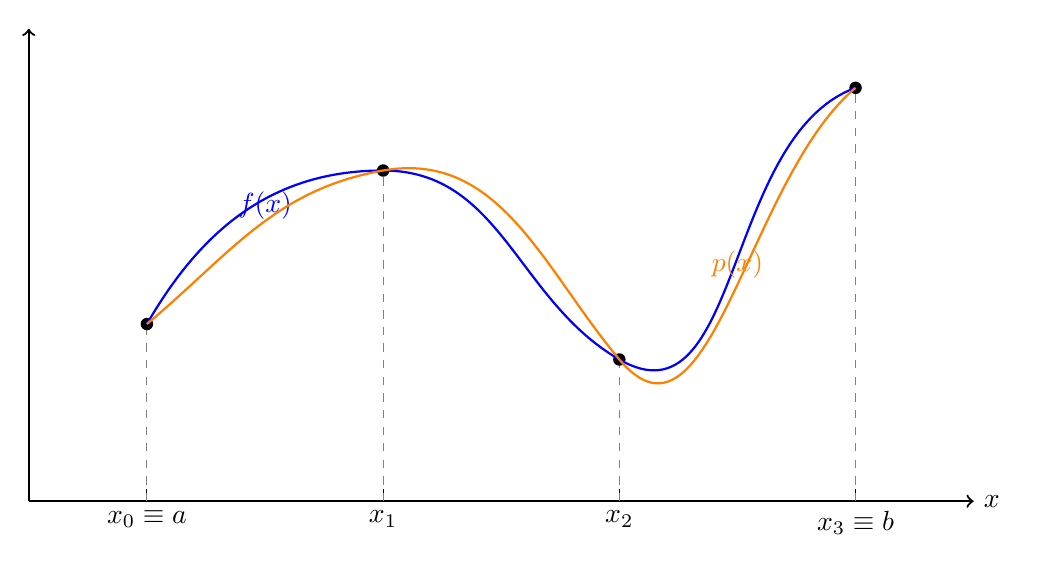
\begin{tikzpicture}[scale=1.5]
    % Assi
    \draw[->, thick] (0,0) -- (8,0) node[right] {$x$};
    \draw[->, thick] (0,0) -- (0,4);
    
    % Nodi
    \draw (1,0) node[below] {$x_0 \equiv a$} -- (1,0.1);
    \draw (3,0) node[below] {$x_1$} -- (3,0.1);
    \draw (5,0) node[below] {$x_2$} -- (5,0.1);
    \draw (7,0) node[below] {$x_3 \equiv b$} -- (7,0.1);
    
    % Linee tratteggiate e punti di intersezione
    \draw[dashed, gray] (1,0) -- (1,1.5);
    \fill[black] (1,1.5) circle (1.5pt);
    
    \draw[dashed, gray] (3,0) -- (3,2.8);
    \fill[black] (3,2.8) circle (1.5pt);
    
    \draw[dashed, gray] (5,0) -- (5,1.2);
    \fill[black] (5,1.2) circle (1.5pt);
    
    \draw[dashed, gray] (7,0) -- (7,3.5);
    \fill[black] (7,3.5) circle (1.5pt);

    % Funzione f(x) e p(x)
    \draw[blue, thick] (1,1.5) to[out=60, in=180] (3,2.8) to[out=0, in=150] (5,1.2) to[out=-30, in=200] (7,3.5);
    \node[blue] at (2, 2.5) {$f(x)$};

    \draw[orange, thick] (1,1.5) to[out=40, in=190] (3,2.8) to[out=10, in=130] (5,1.2) to[out=-50, in=220] (7,3.5);
    \node[orange] at (6, 2) {$p(x)$};

\end{tikzpicture}
\end{center}

$p(x)$ è il polinomio interpolante $f(x)$ nelle ascisse assegnate.

\subsubsection{Errore di interpolazione}
Se definiamo (funzione dell'errore):
$$e(x) = f(x) - p(x)$$
ricordando che $p(x_i) = f(x_i)$, $i=0,\dots,n$, otteniamo che:
$$e(x_i) = 0, \quad i=0,\dots,n.$$

Cosa succede se $x \neq x_i$?








%11/03/2026

\vspace{0.4cm}
\begin{teorema}
    L'errore di interpolazione si può esprimere come:
\begin{equation} \label{eq:err1}
    e(x) = f[x_0, \dots, x_n, x] w_{n+1}(x)
\end{equation}
con $w_{n+1}(x) = \prod_{j=0}^{n} (x - x_j)$ che è il polinomio monico le cui radici sono le ascisse di interpolazione.
\end{teorema}


\begin{proof}
Se $x = x_i \implies e(x_i) = 0$, perché $w_{n+1}(x_i) = 0$, $\forall i=0,\dots,n$, quindi la \eqref{eq:err1} è verificata.

Se $x = \hat{x} \notin \{x_0, \dots, x_n\}$, allora, sfruttando la costruzione incrementale del polinomio interpolante di Newton, possiamo definire $\hat{p}(x) \in \Pi_{n+1}$ che interpola $f(x)$ in $x_0, x_1, \dots, x_n, \hat{x}$ come:
\begin{equation} \label{eq:err2}
    \hat{p}(x) = p(x) + f[x_0, \dots, x_n, \hat{x}] w_{n+1}(x)
\end{equation}
Il termine $p(x)$ è il polinomio interpolante in $x_0, \dots, x_n$, mentre l'ultimo termine è il pezzo "aggiuntivo" che dà l'interpolazione in $\hat{x}$.

Pertanto:
$$ \hat{p}(x_i) = f(x_i), \quad i=0, \dots, n $$
e
\begin{equation} \label{eq:err3}
    \hat{p}(\hat{x}) = f(\hat{x})
\end{equation}
ovvero, tenendo conto della \eqref{eq:err2}, si ottiene:
$$ p(\hat{x}) + f[x_0, \dots, x_n, \hat{x}] w_{n+1}(\hat{x}) = f(\hat{x}) $$
Da questo ricaviamo che:
$$ f[x_0, \dots, x_n, \hat{x}] w_{n+1}(\hat{x}) = f(\hat{x}) - p(\hat{x}) \equiv e(\hat{x}) $$
Osservando che $\hat{x}$ è generico, si ottiene, infine:
$$ e(x) = f[x_0, \dots, x_n, x] w_{n+1}(x) $$
ovvero la tesi \eqref{eq:err1}.
\end{proof}

\vspace{0.4cm}
\textbf{Corollario:}
Se $f \in \mathcal{C}^{(n+1)}$ su un intervallo che contiene le ascisse di interpolazione ed il punto $x$ considerato, allora:
\begin{equation} \label{eq:err_cor}
    e(x) = \frac{f^{(n+1)}(\xi_x)}{(n+1)!} w_{n+1}(x)
\end{equation}
con $\xi_x \in I(x_0, \dots, x_n, x)$, avendo denotato con $I(x_0, \dots, x_n, x)$ il più piccolo intervallo che contiene le ascisse in argomento.

\begin{proof}
Infatti, l'equazione \eqref{eq:err_cor} deriva dalla \eqref{eq:err1} che, nelle ipotesi fatte, considerando che:
$$ f[x_0, \dots, x_n, x] = \frac{f^{(n+1)}(\xi_x)}{(n+1)!} $$
con $\xi_x$ opportuno.
\end{proof}

\newpage
\textbf{OSS.}
\begin{enumerate}
    \item Se $f(x) \in \Pi_n \implies f^{(n+1)}(x) \equiv 0 \implies e(x) = f(x) - p(x) \equiv 0$ ovvero, $f(x) \equiv p(x)$, per l'unicità del polinomio interpolante, come già osservato.
    \item Dalla \eqref{eq:err_cor} otteniamo che l'errore $e(x)$ è dato dal prodotto di 2 termini:
    \begin{itemize}
        \item $\frac{f^{(n+1)}(\xi_x)}{(n+1)!}$: questo dipende da quanto è "buona" la funzione $f(x)$. Il fattoriale al denominatore significa che le derivate diventano "piccole" al crescere dell'ordine.
        \item $w_{n+1}(x) = \prod_{i=0}^{n} (x - x_i)$: che dipende esclusivamente dalla scelta delle ascisse di interpolazione.
    \end{itemize}
\end{enumerate}

Tuttavia, se $x \gg \max \{x_i\}$ oppure $x \ll \min \{x_i\}$, allora $w_{n+1}(x) \approx x^{n+1}$ ($w_{n+1}(x)$ diventa molto grande al crescere di $n$). Pertanto, $p(x)$ è un'approssimazione "spendibile" di $f(x)$ solo se $x$ è prossimo (meglio se all'interno) dell'intervallo che contiene le ascisse di interpolazione.

\begin{center}
    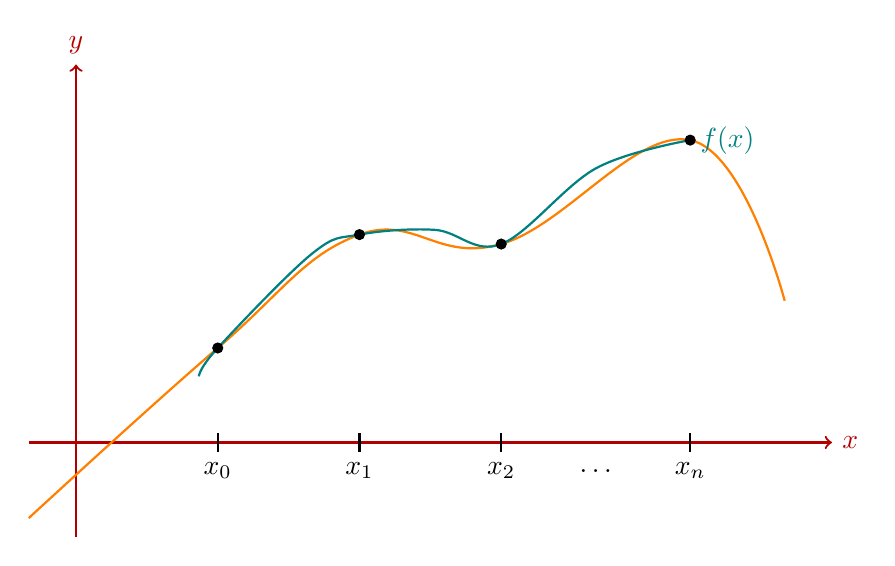
\begin{tikzpicture}[scale=1.2]
        % Assi
        \draw[->, thick, red!70!black] (-0.5,0) -- (8,0) node[right] {$x$};
        \draw[->, thick, red!70!black] (0,-1) -- (0,4) node[above] {$y$};
        
        % Punti x_i
        \draw[thick] (1.5, 0.1) -- (1.5, -0.1) node[below] {$x_0$};
        \draw[thick] (3, 0.1) -- (3, -0.1) node[below] {$x_1$};
        \draw[thick] (4.5, 0.1) -- (4.5, -0.1) node[below] {$x_2$};
        \node at (5.5, -0.3) {$\dots$};
        \draw[thick] (6.5, 0.1) -- (6.5, -0.1) node[below] {$x_n$};
        
        % Polinomio p(x) in arancione
        \draw[orange, thick] plot [smooth, tension=0.7] coordinates {(-0.5,-0.8) (1.5,1) (3,2.2) (4.5,2.1) (6.5,3.2) (7.5,1.5)};
        
        % Funzione f(x) in verde scuro
        \draw[teal, thick] plot [smooth, tension=0.6] coordinates {(1.3,0.7) (1.5,1) (2.5,2.0) (3,2.2) (3.8,2.25) (4.5,2.1) (5.5,2.9) (6.5,3.2)} node[right] {$f(x)$};
        
        % Punti di intersezione
        \filldraw[black] (1.5,1) circle (1.5pt);
        \filldraw[black] (3,2.2) circle (1.5pt);
        \filldraw[black] (4.5,2.1) circle (1.5pt);
        \filldraw[black] (6.5,3.2) circle (1.5pt);
    \end{tikzpicture}
    \end{center}

\subsubsection{Interpolazione di Hermite}
Supponiamo, in questo caso, di ricercare il polinomio interpolante, di grado $2n+1$ su $2n+2$ ascisse distinte, che numeriamo come:
$$ x_0 < x_{\frac{1}{2}} < x_1 < x_{1+\frac{1}{2}} < \dots < x_n < x_{n+\frac{1}{2}} $$
Sia $f(x)$ la funzione interpolanda su tali ascisse. Pertanto, sappiamo che $\exists! p(x) \in \Pi_{2n+1}$ tale che:
\begin{equation} \label{eq:hermite1}
    p(x_i) = f(x_i) \quad \text{e} \quad p(x_{i+\frac{1}{2}}) = f(x_{i+\frac{1}{2}}), \quad i=0, \dots, n
\end{equation}

\textbf{Domanda:} Cosa succede a $p(x)$ se $\forall i=0, \dots, n$, si ha $x_{i+\frac{1}{2}} \to x_i$?

Per rispondere correttamente a questa domanda riscriviamo la \eqref{eq:hermite1} come:
$$ p(x_i) = f(x_i) $$
e
\begin{equation} \label{eq:hermite2}
    \frac{p(x_{i+\frac{1}{2}}) - p(x_i)}{x_{i+\frac{1}{2}} - x_i} = \frac{f(x_{i+\frac{1}{2}}) - f(x_i)}{x_{i+\frac{1}{2}} - x_i}, \quad i=0, \dots, n
\end{equation}
A questo punto, se facciamo il limite nella seconda espressione per $x_{i+\frac{1}{2}} \to x_i$, $\forall i=0, \dots, n$, abbiamo dimostrato che $\exists$ un polinomio $p(x) \in \Pi_{2n+1}$ tale che la \eqref{eq:hermite2} diventa:
\begin{equation} \label{eq:hermite3}
    p(x_i) = f(x_i) \quad \text{e} \quad p'(x_i) = f'(x_i), \quad i=0, \dots, n
\end{equation}

\vspace{0.4cm}
\begin{definition}
Il polinomio $p(x) \in \Pi_{2n+1}$ che soddisfa le condizioni di interpolazione \eqref{eq:hermite3} è detto \textbf{polinomio interpolante di Hermite}.
\end{definition}

\textbf{OSS.} In altri termini, il polinomio interpolante di Hermite interpola, nelle ascisse di interpolazione, sia la funzione $f(x)$ che la sua derivata prima. Pertanto ha la stessa retta tangente nelle ascisse di interpolazione.

\begin{center}
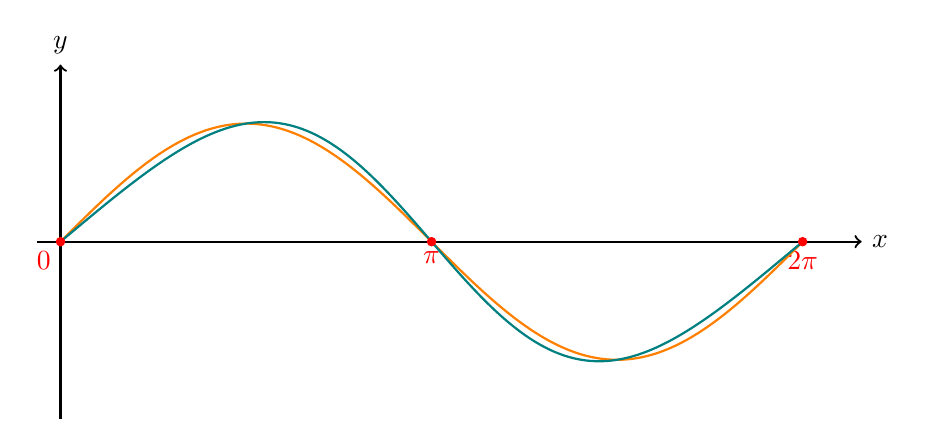
\begin{tikzpicture}[scale=1.5]
    % Assi
    \draw[->, thick] (-0.2, 0) -- (2*pi+0.5, 0) node[right] {$x$};
    \draw[->, thick] (0, -1.5) -- (0, 1.5) node[above] {$y$};
    
    % Punti nodali
    \node[below left, text=red] at (0,0) {$0$};
    \node[below, text=red] at (pi,0) {$\pi$};
    \node[below, text=red] at (2*pi,0) {$2\pi$};
    
    % Funzione f(x) = sin(x) (arancione)
    \draw[orange, thick, smooth, samples=100, domain=0:2*pi] plot (\x, {sin(\x r)});
    
    % Polinomio di Hermite approssimato (verde scuro)
    % (In questo schema grafico il polinomio di Hermite segue la sinusoide quasi perfettamente
    % poiché condivide radici e tangenti, al contrario del polinomio classico che sarebbe identicamente nullo)
    \draw[teal, thick, smooth, samples=100, domain=0:2*pi] plot (\x, {sin(\x r) - 0.08*sin(2*\x r)}); 
    
    % Punti rossi
    \filldraw[red] (0,0) circle (1pt);
    \filldraw[red] (pi,0) circle (1pt);
    \filldraw[red] (2*pi,0) circle (1pt);
\end{tikzpicture}
\end{center}

\vspace{0.4cm}
Se $f(x) = \sin(x)$ e $x_i = i\pi$, per $i=0, 1, 2$, allora il polinomio interpolante (classico) su tali ascisse è zero!
Questo \textbf{non} è vero per il polinomio interpolante di Hermite.
%Vedremo in che modo si possa calcolare efficientemente il polinomio interpolante di Hermite. In particolare, ne vedremo la forma di Newton.









%12/03/2026
\vspace{0.4cm}
Per derivare la forma di Newton di questo polinomio, facciamo un passo indietro considerando, formalmente, le $2n+2$ ascisse:
$$ a \le x_0 < x_{1/2} < x_1 < x_{1+1/2} < \dots < x_n < x_{n+1/2} \le b $$

Fissiamo, ad esempio, il caso $n=2$, abbiamo che il relativo polinomio interpolante è dato da:
\begin{align*}
p(x) &= f[x_0] + f[x_0, x_{1/2}](x-x_0) + f[x_0, x_{1/2}, x_1](x-x_0)(x-x_{1/2}) \\
&\quad + f[x_0, x_{1/2}, x_1, x_{1+1/2}](x-x_0)(x-x_{1/2})(x-x_1) \\
&\quad + f[x_0, x_{1/2}, x_1, x_{3/2}, x_2](x-x_0)(x-x_{1/2})(x-x_1)(x-x_{3/2}) \\
&\quad + f[x_0, x_{1/2}, x_1, x_{3/2}, x_2, x_{5/2}](x-x_0)(x-x_{1/2})(x-x_1)(x-x_{3/2})(x-x_2)
\end{align*}

Se adesso poniamo $x_{1/2} = x_0$, $x_{3/2} = x_1$, $x_{5/2} = x_2$, otteniamo la forma di Newton del polinomio di Hermite corrispondente:
\begin{align*}
    p_H(x) &= f[x_0] + f[x_0, x_0](x-x_0) + f[x_0, x_0, x_1](x-x_0)(x-x_0) \\
    &\quad + f[x_0, x_0, x_1, x_1](x-x_0)(x-x_0)(x-x_1) \\
    &\quad + f[x_0, x_0, x_1, x_1, x_2](x-x_0)(x-x_0)(x-x_1)(x-x_1) \\
    &\quad + f[x_0, x_0, x_1, x_1, x_2, x_2](x-x_0)(x-x_0)(x-x_1)(x-x_1)(x-x_2)
    \end{align*}

\underline{\textbf{OSS}}
\begin{enumerate}
    \item Il calcolo del polinomio, note le differenze divise, si può far agevolmente mediante l'algoritmo di Horner generalizzato, semplicemente duplicando le ascisse di interpolazione.
    \item Il calcolo delle differenze divise, visto che ci sono ascisse ripetute in argomento, richiede qualche modifica invece dell'algoritmo classico per il polinomio interpolante.
\end{enumerate}

A questo fine, costruiamo (formalmente) la tabella triangolare per il calcolo delle differenze divise. Per semplicità, consideriamo il caso $n=1$ che è ancora rappresentativo:

\begin{center}
\renewcommand{\arraystretch}{1.5}
\begin{tabular}{c|cccc}
 & 0 & 1 & 2 & 3 \\
\hline
$x_0$ & $f[x_0]$ & & & \\
$x_0$ & $f[x_0]$ & $f[x_0, x_0]$ & & \\
$x_1$ & $f[x_1]$ & $f[x_0, x_1]$ & $f[x_0, x_0, x_1]$ & \\
$x_1$ & $f[x_1]$ & $f[x_1, x_1]$ & $f[x_0, x_1, x_1]$ & $f[x_0, x_0, x_1, x_1]$ \\
\end{tabular}
\end{center}

Partendo dall'ultima colonna, abbiamo che:
$$ f[x_0, x_0, x_1, x_1] = \frac{f[x_0, x_1, x_1] - f[x_0, x_0, x_1]}{x_1 - x_0} \quad \text{\textcolor{green}{\checkmark}} $$

Passando, quindi, alla penultima colonna, abbiamo che:
$$ f[x_0, x_0, x_1] = \frac{f[x_0, x_1] - f[x_0, x_0]}{x_1 - x_0} \quad \text{\textcolor{green}{\checkmark}} $$
$$ f[x_0, x_1, x_1] = \frac{f[x_1, x_1] - f[x_0, x_1]}{x_1 - x_0} \quad \text{\textcolor{green}{\checkmark}} $$

Passiamo, infine, alla colonna 1:
$$ f[x_0, x_0] = ? \quad \text{\textcolor{red}{\textbf{X}}} $$
$$ f[x_0, x_1] = \frac{f[x_1] - f[x_0]}{x_1 - x_0} \quad \text{\textcolor{green}{\checkmark}} $$
$$ f[x_1, x_1] = ? \quad \text{\textcolor{red}{\textbf{X}}} $$

In conclusione, qualunque sia il valore di $n$ considerato, abbiamo che il problema, nel calcolo delle differenze divise, si manifesta nel calcolo di $f[x_i, x_i]$, $i=0, \dots, n$.
Queste ultime sono definite come segue:
$$ f[x_i, x_i] = \lim_{h \to 0} f[x_i+h, x_i] = \lim_{h \to 0} \frac{f[x_i+h] - f[x_i]}{h} = \lim_{h \to 0} \frac{f(x_i+h) - f(x_i)}{h} = f'(x_i) $$
che è un \textbf{dato del problema}.

Possiamo, a questo punto, formulare un algoritmo modificato per il calcolo delle differenze divise della forma di Newton del polinomio di Hermite. Necessitiamo di 2 vettori, di lunghezza $2n+2$, che contengono i dati del problema:
$$ f = [f_0, f'_0, f_1, f'_1, \dots, f_n, f'_n] $$
$$ x = [x_0, x_0, x_1, x_1, \dots, x_n, x_n] $$

\begin{verbatim}
% Colonna 1
for i = 2*n+1 : -2 : 3
    f(i) = (f(i) - f(i-2)) / (x(i) - x(i-1));
end

for j = 2 : 2*n+1
    for i = 2*n+2 : -1 : j+1
        f(i) = (f(i) - f(i-1)) / (x(i) - x(i-j));
    end
end
\end{verbatim}

\vspace{0.4cm}
\subsubsection*{Calcolo di un polinomio e della sua derivata prima, espresso nella base di Newton.}
\begin{equation} \label{eq:newt_deriv}
p(x) = \sum_{i=0}^{n} a_i w_i(x)
\end{equation}
$$
\begin{cases}
w_i(x) = w_{i-1}(x)(x - x_{i-1}) \\
w_0(x) = 1
\end{cases}
$$

Avevamo visto l'algoritmo di Horner generalizzato per il calcolo di \eqref{eq:newt_deriv}:
\begin{verbatim}
p1 = 0;                  % AGGIUNTO per calcolare p'(x)
p = a_n;
for i = n-1 : -1 : 0
    p1 = p1 * (x - x_i) + p;    % AGGIUNTO per calcolare p'(x)
    p = p * (x - x_i) + a_i;
end
\end{verbatim}
Come abbiamo visto, `p` alla fine conterrà il valore di $p(x)$. Aggiungiamo (le righe commentate) nel precedente pseudocodice il calcolo di `p1` che, alla fine, conterrà il valore di $p'(x)$. In questo modo, nello stesso ciclo, si calcola sia il valore di $p(x)$ che della sua derivata prima.

\vspace{0.6cm}
\subsection*{Forma di Lagrange del polinomio interpolante di Hermite}
Dati:
$$ a \le x_0 < x_1 < \dots < x_n \le b $$
$$ f_i = f(x_i), \quad f'_i = f'(x_i) \quad i=0, \dots, n $$
Abbiamo detto che $\exists p_H(x) \in \Pi_{2n+1}$ tale che:
$$ p_H(x_i) = f_i $$
$$ p'_H(x_i) = f'_i, \quad i=0, \dots, n $$
Vediamo come ottenere la forma di Lagrange. A questo fine, ricordiamo i polinomi di Lagrange di grado $n$:
$$ L_{in}(x) = \prod_{\substack{j=0 \\ j \neq i}}^{n} \frac{x - x_j}{x_i - x_j}, \quad i=0, \dots, n $$
Ricordiamo, inoltre, che $L_{in}(x_k) = \delta_{ik} = \begin{cases} 1, & i=k \\ 0, & i \neq k \end{cases}$

Definiamo, quindi, i seguenti polinomi di grado $2n+1$:
\begin{equation} \label{eq:lagrange_hermite}
\begin{cases}
\Phi_{in}(x) = L_{in}^2(x) [1 - 2(x - x_i)L'_{in}(x_i)] \\
\Psi_{in}(x) = (x - x_i)L_{in}^2(x)
\end{cases} \quad i=0, \dots, n
\end{equation}

\textbf{Es.} Calcolare l'espressione di $L'_{in}(x_i)$.

\vspace{0.2 cm}
\textbf{Svolgimento (GEMINI):}
Partiamo dalla definizione del polinomio base di Lagrange:
$$ L_{in}(x) = \prod_{\substack{j=0 \\ j \neq i}}^{n} \frac{x - x_j}{x_i - x_j} $$

Possiamo riscriverlo separando la parte dipendente da $x$ (il numeratore) dalla costante (il denominatore):
$$ L_{in}(x) = \frac{1}{C_i} \prod_{\substack{j=0 \\ j \neq i}}^{n} (x - x_j) $$
dove $C_i = \prod_{\substack{j=0 \\ j \neq i}}^{n} (x_i - x_j)$.

Calcoliamo ora la derivata prima $L'_{in}(x)$ applicando la regola di derivazione del prodotto (la derivata di un prodotto di fattori è la somma dei prodotti in cui un fattore alla volta viene derivato, e la derivata di $(x-x_j)$ è $1$):
$$ L'_{in}(x) = \frac{1}{C_i} \sum_{\substack{k=0 \\ k \neq i}}^{n} \left( 1 \cdot \prod_{\substack{j=0 \\ j \neq i \\ j \neq k}}^{n} (x - x_j) \right) $$

Valutiamo questa espressione nel punto $x = x_i$:
$$ L'_{in}(x_i) = \frac{1}{C_i} \sum_{\substack{k=0 \\ k \neq i}}^{n} \prod_{\substack{j=0 \\ j \neq i \\ j \neq k}}^{n} (x_i - x_j) $$

Osserviamo attentamente la produttoria dentro la sommatoria: essa contiene tutti i termini di $C_i$ tranne quello in cui $j=k$. Possiamo quindi riscriverla come una divisione:
$$ \prod_{\substack{j=0 \\ j \neq i \\ j \neq k}}^{n} (x_i - x_j) = \frac{\prod_{\substack{j=0 \\ j \neq i}}^{n} (x_i - x_j)}{x_i - x_k} = \frac{C_i}{x_i - x_k} $$

Sostituendo questa relazione nella formula della derivata, otteniamo:
$$ L'_{in}(x_i) = \frac{1}{C_i} \sum_{\substack{k=0 \\ k \neq i}}^{n} \frac{C_i}{x_i - x_k} $$

Semplificando la costante $C_i$ al numeratore e al denominatore, si giunge al risultato finale:
$$ L'_{in}(x_i) = \sum_{\substack{k=0 \\ k \neq i}}^{n} \frac{1}{x_i - x_k} $$

\begin{teorema}
    Con riferimento ai polinomi in \eqref{eq:lagrange_hermite}, valgono le seguenti proprietà per ogni $j=0, \dots, n$:
    \begin{equation} \label{eq:prop_lagrange}
    \begin{cases}
    \Phi_{in}(x_j) = \delta_{ij} \\
    \Phi'_{in}(x_j) = 0
    \end{cases}
    \qquad \text{e} \qquad
    \begin{cases}
    \Psi_{in}(x_j) = 0 \\
    \Psi'_{in}(x_j) = \delta_{ij}
    \end{cases}
    \end{equation}
    \end{teorema}
    
    \begin{proof}
    (GEMINI) Ricordiamo la proprietà fondamentale della base di Lagrange: $L_{in}(x_j) = \delta_{ij}$, ovvero vale $1$ se $i=j$ e $0$ se $i \neq j$.
    
    \textbf{1. Dimostriamo le proprietà di $\Psi_{in}(x)$:}
    Partiamo dalla definizione:
    $$ \Psi_{in}(x) = (x - x_i)L_{in}^2(x) $$
    
    Calcoliamo $\Psi_{in}(x_j)$:
    \begin{itemize}
        \item Se $j \neq i$: $L_{in}(x_j) = 0 \implies \Psi_{in}(x_j) = (x_j - x_i) \cdot 0^2 = 0$.
        \item Se $j = i$: $\Psi_{in}(x_i) = (x_i - x_i)L_{in}^2(x_i) = 0 \cdot 1^2 = 0$.
    \end{itemize}
    Quindi $\Psi_{in}(x_j) = 0$ per ogni $j$.
    
    Calcoliamo ora la derivata $\Psi'_{in}(x)$ con la regola del prodotto:
    $$ \Psi'_{in}(x) = 1 \cdot L_{in}^2(x) + (x - x_i) \cdot 2L_{in}(x)L'_{in}(x) $$
    Valutiamola in $x_j$:
    \begin{itemize}
        \item Se $j \neq i$: $L_{in}(x_j) = 0$, quindi entrambi gli addendi si annullano $\implies \Psi'_{in}(x_j) = 0$.
        \item Se $j = i$: il secondo addendo si annulla per il termine $(x_i - x_i)=0$, e rimane $\Psi'_{in}(x_i) = L_{in}^2(x_i) = 1^2 = 1$.
    \end{itemize}
    Quindi $\Psi'_{in}(x_j) = \delta_{ij}$.
    
    \vspace{0.3cm}
    \textbf{2. Dimostriamo le proprietà di $\Phi_{in}(x)$:}
    Partiamo dalla definizione:
    $$ \Phi_{in}(x) = [1 - 2(x - x_i)L'_{in}(x_i)] L_{in}^2(x) $$
    
    Calcoliamo $\Phi_{in}(x_j)$:
    \begin{itemize}
        \item Se $j \neq i$: $L_{in}(x_j) = 0 \implies \Phi_{in}(x_j) = [\dots] \cdot 0^2 = 0$.
        \item Se $j = i$: $L_{in}(x_i) = 1$, quindi $\Phi_{in}(x_i) = [1 - 2(x_i - x_i)L'_{in}(x_i)] \cdot 1^2 = [1 - 0] \cdot 1 = 1$.
    \end{itemize}
    Quindi $\Phi_{in}(x_j) = \delta_{ij}$.
    
    Infine, calcoliamo la derivata $\Phi'_{in}(x)$ applicando la regola del prodotto (notando che $-2L'_{in}(x_i)$ è una costante numerica):
    $$ \Phi'_{in}(x) = \left[ -2L'_{in}(x_i) \right] L_{in}^2(x) + [1 - 2(x - x_i)L'_{in}(x_i)] \cdot 2L_{in}(x)L'_{in}(x) $$
    Valutiamola in $x_j$:
    \begin{itemize}
        \item Se $j \neq i$: $L_{in}(x_j) = 0$, quindi tutti i termini contenenti $L_{in}$ si annullano $\implies \Phi'_{in}(x_j) = 0$.
        \item Se $j = i$: sostituiamo $x_i$ al posto di $x$ e usiamo $L_{in}(x_i) = 1$:
        \begin{align*}
            \Phi'_{in}(x_i) &= -2L'_{in}(x_i) \cdot 1^2 + [1 - 2(0)L'_{in}(x_i)] \cdot 2(1)L'_{in}(x_i) \\
            &= -2L'_{in}(x_i) + [1] \cdot 2L'_{in}(x_i) \\
            &= -2L'_{in}(x_i) + 2L'_{in}(x_i) = 0
        \end{align*}
    \end{itemize}
    Quindi $\Phi'_{in}(x_j) = 0$ per ogni $j$.
    \end{proof}

\vspace{0.4cm}
Dalle \eqref{eq:prop_lagrange} discende che:
\begin{equation} \label{eq:lagrange_final}
p_H(x) = \sum_{i=0}^{n} [f_i \Phi_{in}(x) + f'_i \Psi_{in}(x)]
\end{equation}
Infatti, $\forall j=0, \dots, n$:
$$ p_H(x_j) = \sum_{i=0}^{n} [f_i \underbrace{\Phi_{in}(x_j)}_{\delta_{ij}} + f'_i \underbrace{\Psi_{in}(x_j)}_{0}] = f_j $$
e, inoltre:
$$ p'_H(x_j) = \sum_{i=0}^{n} [f_i \underbrace{\Phi'_{in}(x_j)}_{0} + f'_i \underbrace{\Psi'_{in}(x_j)}_{\delta_{ij}}] = f'_j $$
Pertanto, sono verificate le condizioni di interpolazione. La \eqref{eq:lagrange_final} è la forma di Lagrange del polinomio interpolante di Hermite.